\subsection{Analisi}

\subsubsection{Prospetto orario}
Nel periodo di analisi la distribuzione oraria è la seguente:

\renewcommand{\arraystretch}{1.4}
\begin{table}[H]
\begin{center}
\begin{tabular}{|c|c|c|c|c|c|c|c|}
\hline
\rowcolor{title_row}
\textbf{\color{title_text}{Nome}} & \textbf{\color{title_text}{Resp.}} & \textbf{\color{title_text}{Ammi.}} & \textbf{\color{title_text}{Analist.}} & \textbf{\color{title_text}{Progett.}} & \textbf{\color{title_text}{Program.}} & \textbf{\color{title_text}{Verific.}} & \textbf{\color{title_text}{Totale}} \\ \hline
Andrea Trevisin  & 6 & 2 & 10 & & & 6 & 24  \\ \hline
Giacomo Barzon   & 4 & 3 & 12 & & & 4 & 23  \\ \hline
Giovanni Sorice  & & 3 & 14 & & & 5 & 22  \\ \hline
Lorenzo Busin    & & 8 & 8 & & & 6 & 22  \\ \hline
Marco Costantino & 5 & 5 & 10 & & & 3 & 23 \\ \hline
Michele Roverato & 9 & 4 & 7 & & & 2 & 22 \\ \hline
Nicolò Tartaggia & 5 & & 8 & & & 10 & 23  \\ \hline
\end{tabular}
\caption{Tabella 5.1.1: Distribuzione oraria del periodo "Analisi"\label{}}
\end{center}
\end{table}
\renewcommand{\arraystretch}{1}

Il seguente grafico dà una rappresentazione visiva della suddivisione oraria: \\
\begin{figure} [H]
	\centering
	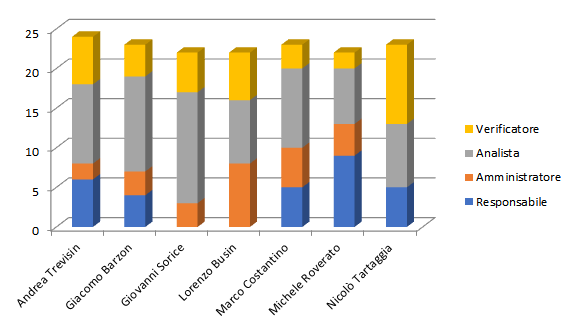
\includegraphics[scale=0.8]{Res/ExcelGrafici/Grafici/AnalisiOre.png}
	\caption{Figura 5.1.1: Grafico suddivisione oraria del periodo "Analisi"}\label{}
\end{figure}


\subsubsection{Prospetto economico}
Nel periodo di analisi il resoconto della distribuzione delle ore e dei relativi costi è la seguente:

\renewcommand{\arraystretch}{1.5}
\begin{table}[H]
\begin{center}
\begin{tabular}{|c|c|c|}
\hline
\rowcolor{title_row}
\textbf{\color{title_text}{Ruolo}}  & \textbf{\color{title_text}{Ore}} & \textbf{\color{title_text}{Costo in \euro}} \\ \hline
Responsabile    & 29           & 870                 \\ \hline
Amministratore  & 25           & 500                 \\ \hline
Analista        & 69           & 1.725                \\ \hline
Progettista     &              &                     \\ \hline
Programmatore   &              &                     \\ \hline
\gl{Verificatore}    & 36           & 540                 \\ \hline
\textbf{Totale} & \textbf{159}    & \textbf{3.635}    \\ \hline
\end{tabular}
\caption{Tabella 5.1.2: Prospetto economico del periodo "Analisi"\label{}}
\end{center}
\end{table}
\renewcommand{\arraystretch}{1}

Il seguente grafico dà una rappresentazione visiva della distribuzione dei ruoli: \\
\begin{figure} [H]
	\centering
	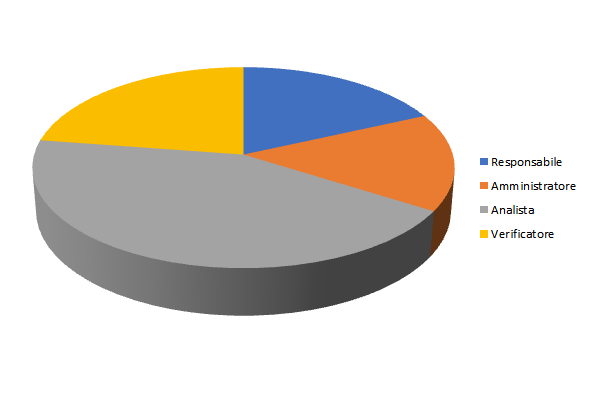
\includegraphics[scale=1]{Res/ExcelGrafici/Grafici/AnalisiRuoli.png}
	\caption{Figura 5.1.2: Grafico suddivisione dei ruoli del periodo "Analisi"}\label{}
\end{figure}

\pagebreak
